\subsection{Festival}
The \href{https://www.trifork.com/news/roskilde-festival}{Trifrok Festival} application is an existing App developed for Android and iOS, Figure \ref{fig:relai_layout}. It allows festival participants to see the concert schedule and other centrally updated information as well as distribution of user-created content. The application has been operational for years while each year new features have been added. The specific use case we are addressing here is the ability to conduct polls where participants can vote for a concert. The challenge is that we cannot see if we receive a vote twice, we don't know who the vote came from, and we do not have a reliable network with a \gls{dc} in the middle.
\begin{figure*}[!ht]
	\centering
	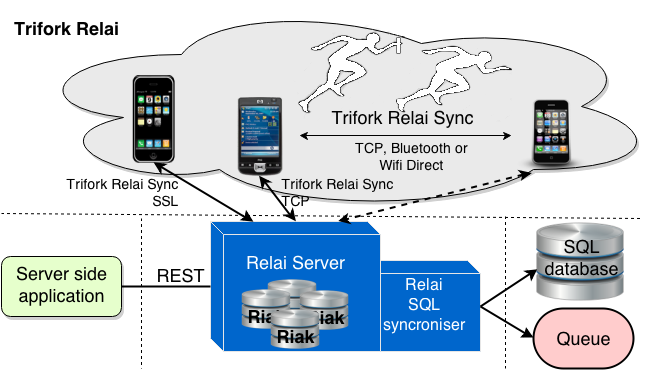
\includegraphics[width=1\textwidth]{figures/TriforkRelai.png}
	
	\caption{Overview of current Festival implementation which uses Trifork's Relai.}
	\label{fig:relai_layout}
\end{figure*}

Massive events like conferences, sport events, and music festivals encounters may saturate the mobile bandwidth which would result in loss of cellular radio connectivity. Based on Trifork Relai local data are updated via not only cellular radio connectivity but also Blue-tooth and WiFi Direct with other devices in a peer-to-peer fashion. So although you may not be able to connect to a \gls{dc} you can still post your votes to peer devices just as you can get more up to date data from these.

Having a normal counter where you add one or more at the time will obviously not work in this scenario as we don't have a central database, we have no means to check how many times you are voting, nor do we have any means to see how large a percentage of possible votes have been given. This raises a new dilemma where the probabilistic counter comes in handy.

Each device will hold a bit array for voting bad and for voting good for each concert, i.e. when a vote is cast as ``bad'' a random number is generated on the device and the corresponding bit in the ``bad'' array is set. The same goes for the ``good'' votes, but note that each possible candidate (bad or good in this case) must have their own bit array. Now this array can be spread to peer devices where it is added to other device\textquoteright s bit arrays as a simple AND operation. At any device you can now see the total number of votes for bad and good by calculating the number of votes that are most likely with number of set bits compared to the number of still unset bits. This value will not change if an array is added several times, in other words it is idempotent. 

One consistency issue that is left unresolved is that you cannot see that few or many votes are missing. Obviously the precision of the count must be obtained by sizing the array towards the total number of votes cast. Another possible inconsistency is that segregated groups of devices can show uncorrelated results. This can happen in a number of situations which are unlikely but possible, i.e. lets say no cellular radio network is available and one group are now only networking using WiFi Direct and another group are only networking using Blue-tooth and no device is bridging the two means of networking. Then each group will have their own voting polls.

We have a number of unintended side effects. For a music festival this is acceptable, while for an App for parliament this would not be acceptable. In the implementation each device can only vote for each concert once and you cannot alter your vote after it has been given. If you have more devices you also have more votes. If you uninstall and reinstall the App you will be able to vote again for the same concert.

\subsubsection{Mark-Counter}
A Mark-Counter is composed of an array of $n$ bits. A Mark-Counter $B$ is composed of $n$ bits each represented by $B_{i} \in \{0, 1\} \forall i \in \{1,\dots, n\}$. $A^{n}$ represents the group of all the arrays of bits of size $n$ ($|B| = n$), where $n$ is also the number of bits in a Mark-Counter.

Bitwise OR operator is represented as | in this document.

{\bf Operations}:
\begin{itemize}
	\item Set a bit in a Mark-Counter: a bit may change individually from 0 to 1 but may not be reset back to zero by this operator.
	
	\item Merge Mark-Counters (bitwise OR operator, |): given two Mark-Counters $B, C \in A^{n}$, their merger is defined as $D = \{D_{i} = B_{i} | C_{i}, i \in \{1,\dots, n\}\}$.
	
	If both arrays have different sizes, i.e. $|B|$ and $|C|$, then $D = \{D_{i} = B_{i} | C_{i}, i \in \{1,\dots, \max{\{|B|, |C|\}}\} \text{ with } B_{j} = 0 ~ \forall ~ j > |B|, C_{k} = 0 ~ \forall ~ k > |C|\}$ and the size of $D$ would be $|D| = \max{\{|B|, |C|\}}$.
	
	\item Count: given a Mark-Counter $B$ the count corresponds to the number of bits that have been set to 1, $\sum^{|B|}_{i = 1} B_{i}$. Similarly, once it is know the number of 1s it is also known the number of zeros for a given array size.
\end{itemize}


{\bf A Mark-Counter is a \gls{crdt}}: A Mark-Counter is a simple data structure which complies with the requirements to be a \gls{crdt}, as shown below.
\begin{itemize}
	\item {\bf Commutative}. Given two Mark-Counts $B$ and $C$ with $n$ bits each where a bit index is presented by $i$ and its value in the Mark-Counter by $B_{i}$ and $C_{i}$ respectively the the merging of the corresponding bit at position $i$ provide the same result irrespective of the order the bit in each Mark-Counter is executed, as shown by, Equation \ref{eq:bit-counter_conmmutative}.
		\begin{equation}
			B_{i} | C_{i} = C_{i} | B_{i}
			\label{eq:bit-counter_conmmutative}
		\end{equation}
		
		The prove is shown on the Table \ref{tab:bit-counter_conmmutative} where the two first columns contain the input Mark-Counters and the last two columns the different order they may be computed which provide the same results.
		\begin{table}[!ht]
			\centering
			\begin{tabular}{|c|c||c|c|}
				\hline
				\multicolumn{2}{|c||}{Values} & \multicolumn{2}{|c|}{Results} \\
				\hline
				$B_{i}$ & $C_{i}$ & $B_{i}|C_{i}$ & $C_{i}|B_{i}$ \\
				\hline
				\hline
				0         & 0          & 0                  & 0             \\
				\hline
				1         & 0          & 1                  & 1             \\
				\hline
				0         & 1          & 1                  & 1             \\
				\hline
				1         & 1          & 1                  & 1             \\
				\hline
			\end{tabular}
			
			\caption{Mark-Counter commutative prove, $i \in \{1,\dots, n\}$.}
			\label{tab:bit-counter_conmmutative}
		\end{table}

	\item {\bf Associative}, Equation \ref{eq:bit-counter_associative}.
		\begin{equation}
			(B_{i} | C_{i}) | D_{i} = B_{i} | (C_{i} | D_{i})
			\label{eq:bit-counter_associative}
		\end{equation}
		
		The prove is shown on the Table \ref{tab:bit-counter_associative}.
		\begin{table}[!ht]
			\centering
			\begin{tabular}{|c|c|c||c|c||c|c|}
				\hline
				\multicolumn{3}{|c||}{Values} & \multicolumn{2}{|c||}{Intermediate} & \multicolumn{2}{|c|}{Results} \\
				\hline
				$B_{i}$ & $C_{i}$ & $D_{i}$ & $B_{i}|  C_{i}$ & $C_{i} | D_{i}$ & ($B_{i} | C_{i}) | D_{i}$ & $B_{i} | (C_{i}) | D_{i})$ \\
				\hline
				\hline
				0         & 0          & 0          & 0                    & 0                    & 0                                 & 0             \\
				\hline
				1         & 0          & 0          & 1                    & 0                    & 1                                 & 1             \\
				\hline
				0         & 1          & 0          & 1                    & 1                    & 1                                 & 1             \\
				\hline
				1         & 1          & 0          & 1                    & 1                    & 1                                 & 1             \\
				\hline
				0         & 0          & 1          & 0                    & 1                    & 1                                 & 1             \\
				\hline
				1         & 0          & 1          & 1                    & 1                    & 1                                 & 1             \\
				\hline
				0         & 1          & 1          & 1                    & 1                    & 1                                 & 1             \\
				\hline
				1         & 1          & 1          & 1                    & 1                    & 1                                 & 1             \\
				\hline
			\end{tabular}
			
			\caption{Mark-Counter associative prove, $i \in \{1,\dots, n\}$.}
			\label{tab:bit-counter_associative}
		\end{table}

	\item {\bf Idempotent}, Equation \ref{eq:bit-counter_idempotent}.
		\begin{equation}
			B_{i} | B_{i} = B_{i}
			\label{eq:bit-counter_idempotent}
		\end{equation}
		
		The prove is shown on the Table \ref{tab:bit-counter_idempotent}.
		\begin{table}[!ht]
			\centering
			\begin{tabular}{|c||c|c|c|}
				\hline
				Value   & Result             \\
				\hline
				$B_{i}$ & $B_{i} | B_{i} $ \\
				\hline
				\hline
				0         & 0                     \\
				\hline
				1         & 1                     \\
				\hline
			\end{tabular}
			
			\caption{Mark-Counter idempotent prove, $i \in \{1,\dots, n\}$.}
			\label{tab:bit-counter_idempotent}
		\end{table}
\end{itemize}


\subsubsection{Festival use case with Mark-Counters} \\
Consider a "Festival" which it is composed of many acts/events. We start by considering the case of a "Festival" composed only of one act that later will be extended to many. To simplify, without losing generality, it is considered the case of an event in a theatre and the constants and variables used are presented in Table \ref{tab:festival_constants_variables}.
\begin{table*}[!ht]
	\begin{tabular}{|p{2.4cm}|p{13.4cm}|r| }
		\hline
		\multicolumn{1}{|c|}{Name} & \multicolumn{1}{c|}{Description} & \multicolumn{1}{c|}{Type} \\
		\hline
		\hline
			$DC$ & It is the group of \glspl{dc} through which an event must be distributed and $d$ identifies one of the \gls{dc}, $d \in \{1,\dots, |DC|\}$. & $\mathbb{Z}_{+}$ \\
		\hline
			$People$ & It is the group of people attending the "Festival", with $|People|$ representing the number of people attending and the size of the array of bits. & $\mathbb{Z}_{+}$ \\
		\hline
			$n_{d}$ & It refers to the highest attendee's index to the "Festival" that the device $d$ has information about,  $d \in \{1,\dots, |People|\}$. Also $1 \le n_{d} \le |People| ~ \forall ~ d \in \{1,\dots, |People|\}$. & $\mathbb{Z}_{+}$ \\
		\hline
			$G_{d}$ & It is the array of good votes known by the device $d$ from device $d$ and other devices. $G_{d}$ is an array of bit of size of at least $n_{d}$, with each bit represent a device. $G_{d}$ is a Mark-Counter where a bit is set to 1 if the corresponding attendee, represented by that bit, is set to 1 to state the vote of the attendee as good. & $\mathbb{Z}_{+}$ \\
		\hline 
			$G_{da}$ & It is the value in the array of good votes available at devise $d$ for attendee $a$, presented in Expression \ref{ep:good_values}. Also it can be said to be the bit $a$ in the array of bits $G_{d}$, $a \in \{1,\dots, |People|\}$.
				\begin{equation} \label{ep:good_values}
					0 \le G_{ka} \le 1 ~ \forall k,a \in \{1,\dots, |People|\}
				\end{equation} & 
			$\mathbb{Z}_{+}$ \\
		\hline
			$B_{d}$ & It is the array of bad votes known by device $d$ from device $d$ and other devices. $B_{d}$ is an array of bit of size of at least $n_{d}$, with each bit represent a device. $B_{d}$ is a Mark-Counter where a bit is set to 1 if the corresponding attendee, represented by that bit, is set to 1 to state the vote of the attendee as bad. & $\mathbb{Z}_{+}$ \\
		 \hline
		 	$B_{da}$ & It is the value in the array of bad votes seen by device $d$ for attendee $a$, $B_{da}$, presented in Expression \ref{ep:bad_values}. Also it can be said to be the bit $a$ in the array of bits $B_{d}$, $a \in \{1,\dots, |People|\}$.
				\begin{equation} \label{ep:bad_values}
					0 \le B_{da} \le 1 ~ \forall d, a \in \{1,\dots, |People|\}
				\end{equation} & 
			$\mathbb{Z}_{+}$ \\
		\hline
			$numGood_{d}$ & It is the number of good votes received by the attendee $d$ device, as shown by Equation \ref{eq:local_total_good_votes}. & $\mathbb{Z}_{+}$ \\
		\hline
			$numGood$ & It represents the total number of attendees that voted good, as shown in Equations  \ref{eq:attendee_voted_good} and \ref{eq:total_good_votes}. It is considered that if $n_{d} < |People|$ then $G_{da} = B_{da} = 0 ~ \forall ~ a > n_{d}$. & $\mathbb{Z}_{+}$ \\
		\hline
			$numBad_{d}$ & It is the number of bad votes received by the attendee $d$ device, as shown by Equation \ref{eq:local_total_bad_votes}. & $\mathbb{Z}_{+}$ \\
		\hline
			$numBad$ & It represents the total number of attendees that voted bad, as shown in Equations \ref{attendee_voted_bad} and \ref{eq:total_bad_votes}. & $\mathbb{Z}_{+}$ \\
		\hline
			$numAttendees_{d}$ & It represents the total number of attendees that voted as seen by device/attendee $d$, as shown in Equation \ref{eq:num_votes}. & $\mathbb{Z}_{+}$ \\
		\hline
			$numAttendees$ & It represents the total number of attendees that voted, as shown in Equation \ref{eq:total_num_votes}. & $\mathbb{Z}_{+}$ \\
		\hline
	\end{tabular}
			
	\caption{Festival Constants and Variables.}
	\label{tab:festival_constants_variables}
\end{table*}
\begin{equation} \label{eq:attendee_voted_good}
	\delta^{good}_{d} = \left\{\begin{array}{ll}
		1 & if \sum_{a \in People} G_{da} > 0\\
		0 & otherwise
	\end{array}
	\right.
\end{equation}
\begin{equation} \label{eq:total_good_votes}
	numGood  = \sum_{d \in People} \delta^{good}_{d}
\end{equation}
\begin{equation} \label{eq:local_total_good_votes}
	numGood_{d}  = \sum^{n_{d}}_{a=1} G_{da} ~ \forall ~ d \in \{1,\dots, |People|\}
\end{equation}
\begin{equation} \label{attendee_voted_bad}
	\delta^{bad}_{d} = \left\{\begin{array}{ll}
		1 & if \sum_{d \in People} B_{da} > 0\\
		0 & otherwise
	\end{array}
	\right.
\end{equation}
\begin{equation} \label{eq:total_bad_votes}
	numBad  = \sum_{d \in People} \delta^{bad}_{d}
\end{equation}
\begin{equation} \label{eq:local_total_bad_votes}
	numBad_{d}  = \sum^{n_{d}}_{a=1} B_{da} ~ \forall ~ d \in \{1,\dots, |People|\}
\end{equation}
\begin{equation} \label{eq:num_votes}
	numAttendees_{d}  = \sum^{n_{d}}_{a=1} (G_{da} + B_{da}) ~ \forall ~ d \in \{1,\dots, |People|\}
\end{equation}
\begin{equation} \label{eq:total_num_votes}
	numAttendees  = numGood + numBad
\end{equation}

An attendee may only vote once as expressed in Inequality \ref{ep:vote_not_equal}, but he/she may not vote at all.
\begin{equation} \label{ep:vote_not_equal}
	G_{da} + B_{da} < 2 ~ \forall ~ d \in \{1,\dots, |People|\}, a \in \{1,\dots, n_{k}\}
\end{equation}

A measure of the coherence for the copies between an attendee $a$ and another attendee $j$ can be obtained by calculating the number of bits where both versions of voting differ as expressed in Equation \ref{eq:discrepancy_votes}. All the devices are in sync if $\bigtriangleup numAttendees_{dj} = 0 ~ \forall ~ d, j \in \{1,\dots, |People|\}$.
\begin{multline} \label{eq:discrepancy_votes}
	\bigtriangleup numAttendees_{dj} = \sum_{i \in People} ((G_{di} + G_{ji}) \% 2 + (B_{dj} + B_{ji}) \% 2)\\ \forall ~ d, j \in \{1,\dots, |People|\}
\end{multline}

This can be extended to multiple events/acts by introducing a new index that represent each of these events/acts.

The problem with the real Festival use case is that not all devices may know about all the attendees and even if they did then the size of the bit arrays may be too big to be efficient their use, so Trifork come with the idea of using Statistical Mark-Counter. which are presented in Section \ref{sec:stat_mark_counter}. In Trifork's Festival the counters are reduced in size by using statistics, and each bit is randomly assigned to a customer.

\subsubsection{Statistical Mark-Counter} \label{sec:stat_mark_counter}
To reduce the amount of data transferred between devices and for cases where not all devises may know the total number of attendees it could be used a probabilistic approach. The current Trifork's Festival implementation already uses an statistical Mark-Counter, where the index of an attendee is calculated randomly for a pre-defined size of the poll, $n_{d} = n \le |People| ~ \forall ~ d \in \{1,\dots, n\}$. This means that different attendees may be assigned the same position in the poll, so potentially their votes would equate to a single vote, if they vote equally. So given this the Inequality \ref{ep:vote_less_equal} would not be complied with so it would needs to be removed from the representation to \ref{attendee_voted_bad}.
\begin{equation} \label{ep:vote_less_equal}
	G_{da} + B_{da} \le 2 ~ \forall ~ d, a \in \{1,\dots, n\}
\end{equation}

The size of the array of bits depends of the quality expected from the results extrapolated, whereas larger sizes generally lead to increased precision, e.g. a size equal to the number of attendees will provide the maximum precision. In practice, the size used in a study is determined based on the cost of data collection, storage, transmission, processing, and the need to have sufficient statistical power. Sizes may be chosen in several different ways such as target for the power and target variance of a statistical test.
